%no borrar PREAMBULO
\documentclass[12pt]{article}

\usepackage[top=3.5 cm, bottom=2.5  cm, left=3 cm, right=3 cm]{geometry}
\usepackage{fancyhdr}
\pagestyle{fancy}

\usepackage[hidelinks]{hyperref} %esta opción saca las cajas de colores de los hiperlinks

\fancyfoot[C]{\thepage }  %numera las páginas

\usepackage[utf8]{inputenc}

\usepackage{amsmath,amsfonts,amssymb}
\usepackage{xcolor}
\usepackage{fancyvrb}
\newcommand\verbbf[1]{\textcolor[rgb]{0,0,1}}%comando para colorear el texto en verbatim

%\linespread{1} %por si queremos achicar el espacio entre lineas

\usepackage{tabularx,booktabs}
\usepackage{graphicx}
\usepackage{float} %para que las figuras puedan ponerse en cualquier lado

\usepackage{subcaption}
\usepackage{layout}
\usepackage{multicol}  %para escribir en columnnas 
\usepackage{float}
\usepackage{textcomp}
\usepackage{natbib}
\usepackage{tikz}
\usepackage{multirow} %para cambiar el alto de una fila en una tabla
\tikzset{
  connect/.style = { dashed, gray }
}
\usepackage{pgfplots}
\pgfplotsset{compat=1.8}
\usepackage[english ,spanish]{babel}
\usepackage{latexsym}
\usepackage{verbatim}

%\usepackage{alltt}
\usepackage{indentfirst}

\usepackage{fancybox, calc} 

\usepackage[flushmargin]{footmisc} %para alinear las notas de página

\usepackage{url}
\usepackage{advdate}
\usepackage{wrapfig}
\usepackage{amsthm}
\usepackage[inline]{enumitem} %para hacer listas en una linea, los mismos comandos con *
\newtheorem*{myteo}{Teorema} % la * es para no numerarlos
\newtheorem*{myexample}{Ejemplo}
\newtheorem*{myprop}{Proposición}
\newtheorem*{mylem}{Lema}
\theoremstyle{definition}
\newtheorem*{mydef}{Definición}
\newtheorem{ejer}{Ejercicio}
\newtheorem*{mydefs}{Definiciones}
%\theoremstyle{remark}
\newtheorem*{myobs}{Observación}
\newtheorem*{remark}{Importante}

\renewcommand{\baselinestretch}{1}  %interlineado

\addto\captionsspanish{%
  \renewcommand{\figurename}{Figura}%
}

\newcommand\myText[1]{\text{\scriptsize\tabular[t]{@{}l@{}}#1\endtabular}}
\addto\captionsspanish{%
  \renewcommand{\tablename}{Tabla}%
}

\def \ds {\displaystyle} %define un comando abreviado  
\def\com{“R”}

\usepackage{hyperref}%para referencias de internet con link!
\newcommand*{\fullref}[1]{\hyperref[{#1}]{ \nameref*{#1}}}
%comando \fullref para que ademas del número de capitulo, sección etc. escriba el título del capitulo, sección o lo que sea a lo que estamos haciendo referencia

\newcommand\comentario[1]{\textcolor{red}{#1}}%comentarios en el pdf

\interfootnotelinepenalty=10000 %previene que se pasen a otra página las notas de pie
\raggedbottom 
\addtolength{\topskip}{0pt plus 10pt}
\addtolength{\footnotesep}{0.1mm}

\VerbatimFootnotes%para poder usar Verbatim en las notas de pie

\begin{document}

\fancyhf{}
\pagestyle{fancy}
\lhead{Departamento de Matem\'{a}tica\\Universidad Nacional del Comahue}
\rhead{Matem\'{a}tica 1\\ Licenciatura en Ciencias Biol\'{o}gicas}

%HASTA ACA 




\begin{centering}
\Large{\textbf{Trabajo Práctico N° 4}}\\
\large{\textbf{Soluciones de ejercicios seleccionados}}\\
%\large{\textbf{Números Reales}}\\
\end{centering}
\vspace{1cm}

\noindent
Como hay dos versiones del práctico circulando, ponemos el enunciado del problema antes de la solución.

\section{Extremos, cotas, conjuntos acotados, Intervalos}

\begin{enumerate}
%1
\item \textbf{Ejercicio 1:} Para los siguientes conjuntos determinar, de ser posible:
\begin{multicols}{3}
\begin{itemize}
\setlength\itemsep{0em}
\item Dos cotas superiores.	
\item Dos cotas inferiores.		
\item El supremo.	
\item El ínfimo.
\item El máximo.
\item El mínimo.
\end{itemize}
\end{multicols}
En caso de no ser posible, explicar por qué.
%\begin{multicols}{2}
\begin{itemize}
\setlength\itemsep{0em}
\item Inciso \textit{(g)}: $\{x \in \mathbb{R} / -x^2+ 3x > 1\}$\\
\textbf{R}: Primero tenemos que ver quién es este conjunto. Es decir, para qué valores de $x$ se cumple que $ -x^2+ 3x > 1$\\
\noindent
Despejando:

\begin{centering}
$ -x^2+ 3x > 1$\\
$ -x^2+ 3x - 1>0$\\
\end{centering}
\vspace{0.3cm}

Hay dos maneras de encontrar este conjunto (para luego dar respuesta a este problema). Una es estudiar el signo de las imágenes de la parábola $f(x)=   -x^2+ 3x - 1$ y otra es factorizar el polinomio de la izquierda y estudiar el signo de los factores para tomar la decisión. Vamos a tomar la primera forma.\\
Las raíces de la parábola $f(x)= -x^2+ 3x - 1=0$ son $x_1= 3+ \sqrt{0,8}$ y  $x_2= 3- \sqrt{0,8}$. Como el coeficiente de  $x^2$ es negativo, la parábola tiene las ramas hacia abajo. Es decir, las imágenes de la función son positivas entre las raíces. Como la desigualdad es estricta, este conjunto es el intervalo abierto $(3- \sqrt{0,8}, 3+ \sqrt{0,8})$.  Ahora que tenemos identificado el conjunto podemos dar respuesta a lo solicitado.\\
Como es un intervalo abierto, al no incluir a sus fronteras, no tiene máximo ni mínimo. Sin embargo, es un conjunto acotado. \\
La raíz de la derecha (extremo superior del intervalo) es $3+ \sqrt{0,8}  \thicksim 2,6180$, de modo que cualquier número mayor que este es una cota superior para este conjunto. Por ejemplo, $C = 3; 5; 1000$. Pero el supremo es, precisamente: $3+ \sqrt{0,8}$. Análogamente, $3- \sqrt{0,8}  \thicksim 0,38197$ de modo que cualquier número menor que este es una cota inferior para este conjunto. Por ejemplo, $c = 0; 0,1; -20$. Pero el ínfimo es, precisamente: $3- \sqrt{0,8}$. 

\item  Inciso \textit{(j)}:  $[-3,2] \cup [4, 6]$\\
\textbf{R}: En este caso la unión de estos dos conjuntos produce un nuevo conjunto, también cerrado, que incluye todos los números reales entre $-3$ y $6$ exceptuando los que están entre $2$ y $4$. La cuestión acá es que no hay otra forma de escribir este conjunto: es una unión de dos intervalos. Pero lo importante es que es un \textbf{un único conjunto}. Entonces, si pensamos en que el \textit{mínimo} de un conjunto es el menor elemento que podemos elegir en él, claramente el mínimo es $m = -3$. El número $4$ (que es el mínimo de $[4.6]$ no es mínimo para nuestro conjunto porque hay infinitos números dentro del conjunto (los que están entre $-3$ y $2$ que son menores que él. En cuanto al máximo, con un razonamiento similar, podemos ver que es $M = 6$. Como  \textbf{cota superior}, entonces, podemos elegir cualquier número mayor o igual que $6$ y como  \textbf{cota inferior}, cualquier número menor o igual que $-3$. En este caso el \textit{supremo} es igual al máximo y el \textit{ínfimo} igual al mínimo.

\item  Inciso \textit{(l)}: $\{x \in \mathbb{R} / -x^2+ 3x < 0\}$\\
\textbf{R}: Este problema lo resolvimos en detalle en el  \href{https://youtu.be/yQe628PPYpU}{\textcolor{blue}{ séptimo encuentro virtual}}, disponible en formato pdf también en \href{https://pedco.uncoma.edu.ar/}{\textcolor{blue}{ PEDCO}}.
\end{itemize}

%\vspace{1cm}
%2
\item \textbf{Ejercicio 2:} Analizar si las siguientes proposiciones son verdaderas o falsas, y justificar.
\begin{itemize}
\setlength\itemsep{0em}
\item Inciso \textit{(b)}:Todo conjunto finito es acotado. \\
\textbf{R:} \textbf{Verdadera}. Para mostrar que una afimación con el cuantificador \textbf{todo} es verdadera, tenemos que hacer un razonamiento deductivo. Acá va:\\
Al ser un conjunto finito, los elementos pueden contarse (y uno termina de contar) y por lo tanto, ordenarse. Así, uno obtiene un elemento del conjunto (el primero), que es el menor de todos (el mínimo, $m$) y otro (el último) que es el mayor de todos (el máximo, $M$). Podemos decir entonces que, para todo elemento $x$ de ese conjunto, $m \leq x \leq M$. Por lo tanto, el conjunto es acotado.
\item Inciso \textit{(c)}:Todo conjunto acotado es finito.\\
\textbf{R:} \textbf{Falsa}. Para mostrar que una afimación con el cuantificador \textbf{todo} es falsa, basta con mostrar un contraejemplo. Podría ser el intervalo $(1,4)$: Es acotado, y no es finito. 
\end{itemize}

%5
\item  \textbf{Ejercicio 5:}  Escribir las definiciones anteriores (intervalos abiertos y cerrados) como conjunción o disyunción de proposiciones.
\begin{itemize}
\setlength\itemsep{0em}
\item \textbf{Intervalo abierto} $(a,b) = \{x \in \mathbb{R}/ a < x < b\}$<\\
\textbf{R:} Tenemos que considerar dos proposiciones simples: $p: x > a$ y $q: x < b$ Entonces, el número real $x \in (a,b)$ si $x$ hace verdadera a la proposición compuesta: $p \wedge q$; $x$ es mayor que $a$ y $x$ es menor que $b$.. 
\item \textbf{intervalo cerrado} $[a,b] = \{x \in \mathbb{R}/ a \leq x \leq b\}$. \\
\textbf{R:}Acá hay involucradas cuatro proposiciones simples: $p: x =a$, $q: x >a$, $r: x < b$, $s: x = b$.  Entonces el número real $x \in [a,b]$ si $x$ hace verdadera a la proposicipon compuesta: $(p \vee q) \wedge (r\vee s)$: $x$ es mayor o igual que $a$ y $x$ es menor o igual que $b$.
\end{itemize}

%11
\item  \textbf{Ejercicio 11: }Representar gráficamente y calcular $A \cup B$, $A\cap B$, $A-B$ y $B-A$ siendo:
\begin{itemize}
\setlength\itemsep{0em}
\item  Inciso \textit{(a)}: $A = (-2, 4)$ y $B = (1,5)$
\begin{figure}[H]
\centering
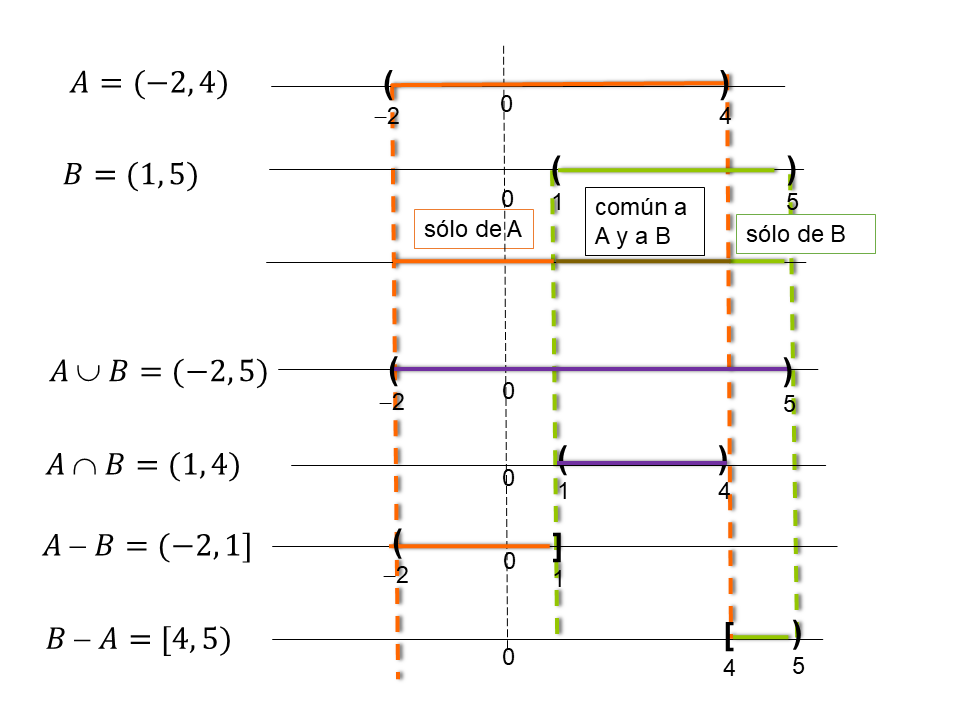
\includegraphics[width=1\textwidth]{11-1.png}
\end{figure}

\item Inciso \textit{(c)}: $A = [-2, 8]$ y $B = (1,5)$
\begin{figure}[H]
\centering
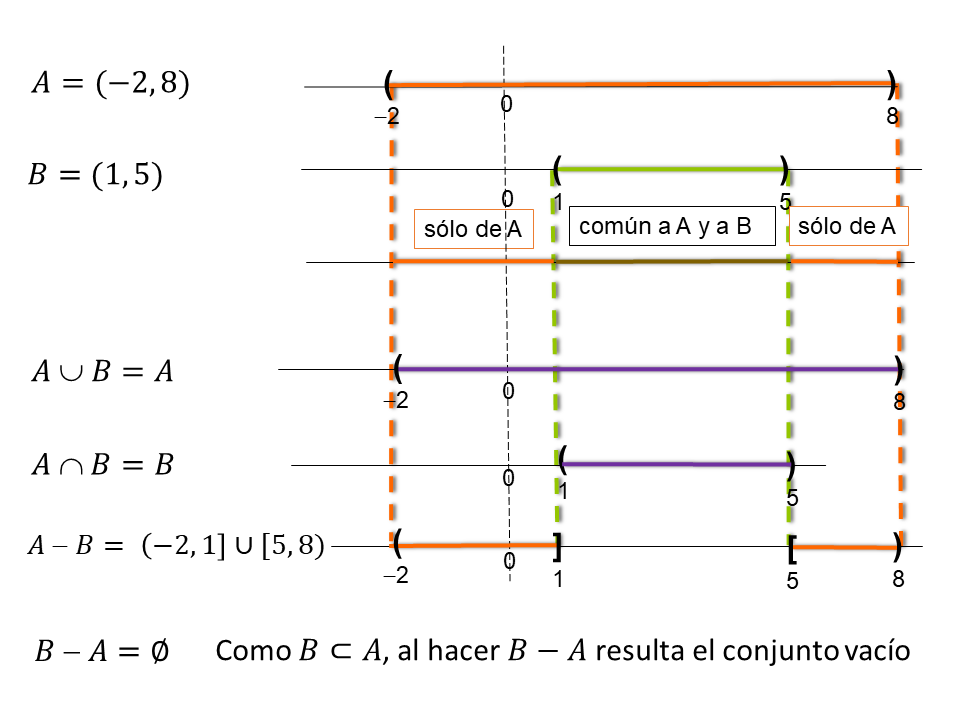
\includegraphics[width=0.85\textwidth]{11-2.png}
\end{figure}

\item Inciso \textit{(e)}:$A = (-1, 4]$ y $B = [4,5)$

\begin{figure}[H]
\centering
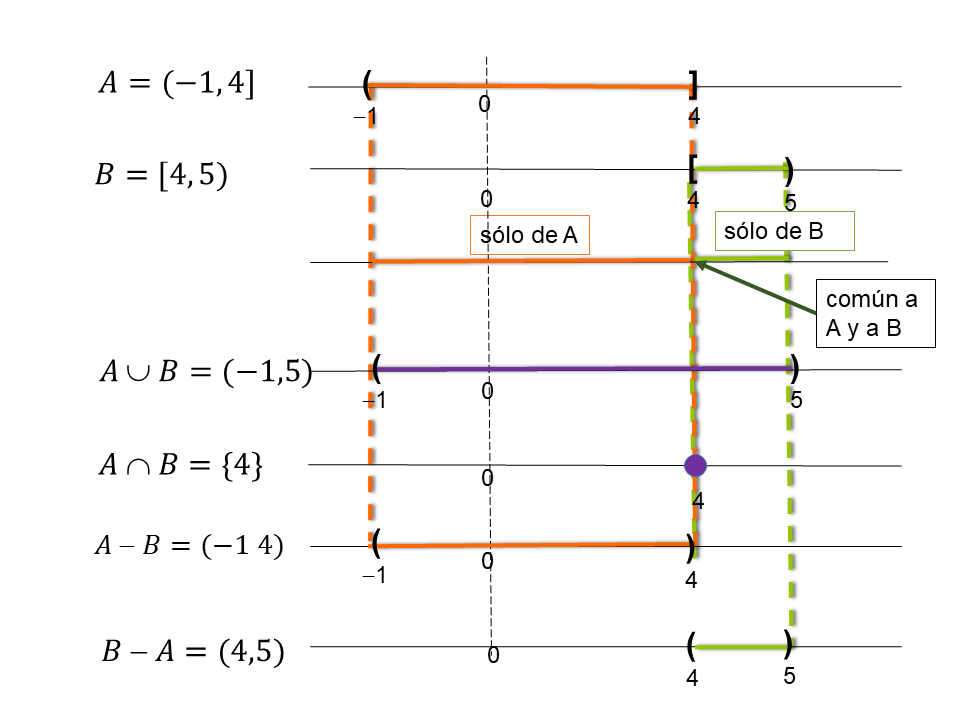
\includegraphics[width=0.85\textwidth]{11-3.png}
\end{figure}

\end{itemize}

%14
\item \textbf{Ejercicio 14:} Analizar si las siguientes proposiciones son verdaderas o falsas, y justificar:
 \begin{itemize}
\setlength\itemsep{0em}
\item Inciso \textit{(c)}: Si una función es acotada (superior e inferiormente), necesariamente tiene máximo y mínimo absolutos.\\
\textbf{R:} \textbf{Falsa}. Para que una función sea acotada sólo se requiere que el conjunto imagen sea acotado. Una función puede tener un intervalo imagen acotado y abierto, como por ejemplo la función del gráfico siguiente:
\begin{figure}[H]
\centering
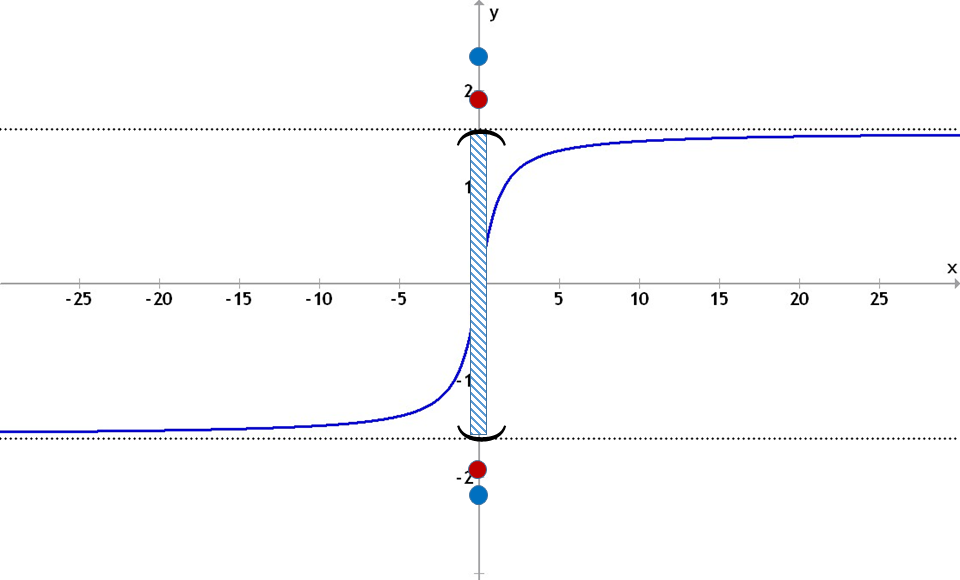
\includegraphics[width=0.85\textwidth]{14-1.png}
\end{figure}
Los puntos sobre el eje vertical son cotas para el conjunto de las imágenes y por lo tanto para la función.
\item Inciso \textit{(c)}: Si una función tiene máximo y mínimo absolutos, necesariamente es acotada.\\
\textbf{R:}\textbf{Verdadera}. Si una función tiene un máximo absoluto $M$, esto significa que para todo $x$ del dominio, se cumple que$f(x) \leq M$. Lo mismo para el mínimo absoluto, llamémoslo $m$, se tiene que para todo $x$ del dominio de la función, $m \leq f(x)$. Por lo tanto, dado que $m \leq f(x) \leq  M$ para todo $x$, la función es acotada.
\end{itemize}


%xxxxxxxxxxxxxxxx FABIAN

\section{Desigualdades. Comparación entre funciones}
%15
\item \textbf{Ejercicio 16:} Para cada uno de los siguientes incisos, llevar a una comparación con cero si no está así, factorizar lo que haga falta y lo que se pueda, y buscar el resultado analizando el signo de cada factor. Escribir los conjuntos solución utilizando intervalos (o unión de ellos):
\begin{enumerate}
	\begin{multicols}{2}
		\item $2 + 3x < 5$
		\item $-2x^2 + 4x \geq 0$
		\item $x^2 - 4 \leq 0$
		\item $\frac{x^2 - 4 }{x(x - 4)} > 0$
		\item $x^3 - 9x^2 > 0$
		\item $(2-x)(3x+2) < 0$
		\item $5x - 2x^2 \leq 3$
		\item $12x^2+6x < x +2$
	\end{multicols}
\end{enumerate}

``Comparar con cero" significa, literalmente, ver si una cantidad es mayor, menor o igual que cero. En el contexto de este ejercicio, partimos de una expresión del tipo $f(x) > g(x)$ (donde el símbolo $>$ puede cambiarse por $<$,$\geq$ o $\leq$ según corresponda), y lo que vamos a hacer primero es transformarla en una desigualdad de tipo $h(x) > 0$ (nuevamente, el símbolo $>$ puede ser diferente). Si hicimos la transformación de forma correcta, la solución de esta nueva desigualdad será igual a la solución de la desigualdad original, y ésta se obtiene simplemente analizando \textit{el signo} de $h(x)$ (es decir, ``comparándola con cero''). Hay varias formas de estudiar el signo de $h(x)$, y si bien la consigna pide explícitamente que lo hagamos ``analizando el signo de cada factor'', veremos además otra forma de resolución que usa argumentos más bien gráficos. Resolveremos detalladamente los primeros dos incisos y sólo daremos las soluciones de los restantes.

\begin{enumerate}
\item $2 + 3x < 5 \implies 2 + 3x - 5 < 0 \implies 3x - 3 < 0 \implies 3(x - 1) < 0$.\\
	
Siguiendo lo explicado en el párrafo anterior, acá $f(x) = 2 + 3x$ y $g(x) = 5$. Trabajamos sobre la expresión y llegamos a $h(x) = 3(x - 1) < 0$. En esta última expresión, tenemos el producto de la constante 3 por el factor lineal $x - 1$, y queremos saber para qué valores de $x$ dicho producto es negativo. Como el número 3 es una constante positiva, el signo del producto será siempre igual al signo de la función $x - 1$. Por lo tanto, la última desigualdad se puede reducir a $x - 1 < 0$, cuya solución es $x < 1$, y en notación de intervalos $x \in (-\infty,1)$. Este procedimiento, que consiste en ``despejar'' $x$ en la desigualdad para hallar el conjunto solución (como hicimos con $x - 1 < 0$), se puede aplicar para cualquier desigualdad en la que estemos comparando una función lineal con cero.\\
	
\item $-2x^2 + 4x \geq 0$.\\
	
\begin{sloppypar}
	En este caso, $g(x) = 0$, por lo que sólo tenemos que hallar el signo de ${f(x) = -2x^2 + 4x}$. Hay dos formas sencillas de hacerlo, y vamos a ver ambas.\\
\end{sloppypar}
	
\textbf{\textit{Forma 1: diagrama de signos}}
	
Factorizamos la función $f(x)$ y analizamos su signo comparando los signos de sus factores:
	
\[-2x^2 + 4x \geq 0 \implies -2x(x - 2) \geq 0.\]
	
En esta última expresión, tenemos el producto de tres factores, a saber, la constante -2 (siempre negativa), el factor lineal $x$ y el factor lineal $x - 2$. El signo del producto se obtiene multiplicando, para cada valor de $x$, los signos de los tres factores. Para hacerlo de forma cómoda y práctica, vamos a usar un ``diagrama de signos'':
	
\begin{figure}[H]
	\centering
	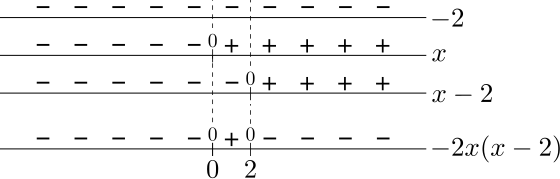
\includegraphics[width=0.6\textwidth]{16_b1.png}
\end{figure}
	
En este diagrama, las líneas horizontales representan la recta real, y cada una de ellas se usa para mostrar el signo de los diferentes factores. Los valores ``importantes'' de $x$ (donde cambia el comportamiento de los diferentes factores) los marcamos en la parte inferior del gráfico (debajo de la línea horizontal inferior), y en este caso son $x = 0$ y $x = 2$. La línea superior muestra el signo del factor $-2$ que, como dijimos, es siempre negativo. El segundo factor, $x$, vale cero para $x = 0$, es positivo cuando $x > 0$ y es negativo cuando $x < 0$. El tercer factor\footnote{Estas conclusiones las sacamos planteando las desigualdades $x - 2 > 0$ y $x - 2 < 0$, respectivamente.}, $x - 2$, vale cero cuando $x = 2$, es positivo cuando $x > 2$ y es negativo cuando $x < 2$. Finalmente, multiplicamos los signos correspondientes para obtener el signo del producto $-2x(x - 2)$, mostrado en la línea inferior. La desigualdad que queríamos resolver es $-2x(x - 2) \geq 0$, y por lo tanto la solución (mirando el gráfico) es $x \in [0,2]$.\\
	
\textbf{\textit{Forma 2: análisis gráfico}}
	
Podemos identificar a la función $f(x) = -2x^2 + 4x$ como una función cuadrática con coeficiente principal negativo. Por lo tanto, sabemos que su gráfico es una parábola con concavidad negativa (``hacia abajo''). Nos interesan los valores de $x$ para los cuales la función es cero o positiva, y por lo tanto dichos valores serán los comprendidos entre sus dos raíces (incluyéndolas), siempre y cuando éstas sean reales. Factorizando (ver \textit{Forma 1}) obtenemos las raíces $x = 0$ y $x = 2$, y la solución es entonces $x \in [0,2]$.
	
\begin{figure}[H]
	\centering
	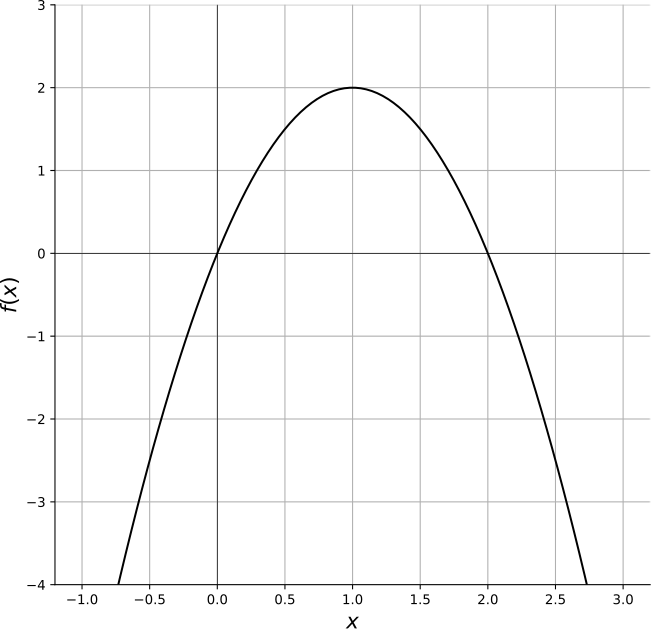
\includegraphics[width=0.6\textwidth]{16_b2.png}
\end{figure}

El análisis gráfico es más rápido que el análisis de los signos, pero sólo resulta útil con algunas funciones. Por ejemplo, para polinomios de grado mayor a 2 o funciones racionales, el análisis de los signos resulta más conveniente.
	
\item Usamos el análisis gráfico. Tenemos una función cuadrática, cuyas raíces son $x = 2$ y $x = -2$ (factorizar, es una diferencia de cuadrados), y la parábola es cóncava hacia arriba (el coeficiente principal es positivo). La desigualdad es $x^2 - 4 \leq 0$, y por lo tanto la solución es $x \in [-2,2]$ (ayudarse haciendo un gráfico a mano alzada).
	
\item Tenemos la desigualdad $\frac{x^2 - 4 }{x(x - 4)} > 0$. En este caso, el análisis de los signos es más adecuado. Recordemos que la regla de los signos se aplica de igual manera en la división y en la multiplicación. En esta función racional, tenemos el denominador factorizado pero el numerador no. Como el numerador es un factor cuadrático, podemos usar el análisis gráfico para saber su signo. Las raíces de $x^2 -4$ son $x = 2$ y $x = -2$, y la parábola es cóncava hacia arriba. Por lo tanto, el diagrama de signos resultante es el siguiente:

\begin{figure}[H]
	\centering
	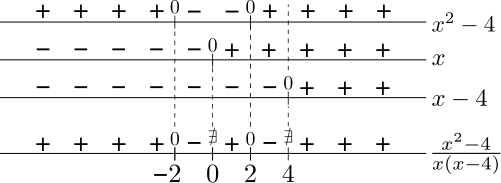
\includegraphics[width=0.6\textwidth]{16_d.png}
\end{figure}
	
La solución es entonces $x \in (\infty,-2) \cup (0,2) \cup (4,+\infty)$. En el diagrama de signos para el cociente, aparece el símbolo $\nexists$ (que significa ``no existe'') en algunos lugares... \textit{¿por qué?}.
	
\item Factorizando: ${x^3 - 9x^2 > 0 \implies x^2(x - 9) > 0}$. En este caso, el problema se simplifica enormemente debido a que el factor $x^2$ es positivo para cualquier valor de $x$. Entonces, el signo del producto viene dado únicamente por el signo del factor lineal $x - 9$, y la desigualdad se reduce a $x - 9 > 0$, cuya solución es $x > 9$, y en notación de intervalos $x \in (9,+\infty)$.
	
\begin{sloppypar}
	\item Tenemos la desigualdad $(3x + 2)(2 - x) < 0$. Usamos el análisis de signos para resolverla. Para el primer factor, como es lineal podemos saber cuándo es positivo resolviendo ${3x + 2 > 0 \implies x > -\frac{2}{3}}$. Para saber cuándo es negativo o cero, basta con cambiar el símbolo $>$ por $<$ o $=$ en esta desigualdad, pero esto lo podemos hacer mentalmente. El signo del segundo factor se determina de la misma manera (también es lineal). El diagrama de signos es entonces:
\end{sloppypar}

\begin{figure}[H]
	\centering
	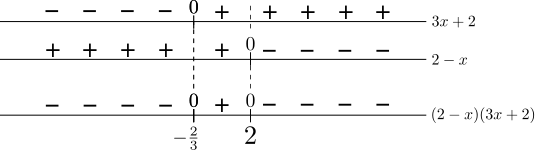
\includegraphics[width=0.8\textwidth]{16_f.png}
\end{figure}
	
La solución es entonces $x \in \left(-\infty,-\frac{2}{3}\right) \cup (2,+\infty)$.
	
\item Tenemos la desigualdad $5x - 2x^2 \leq 3$. En primer lugar vamos a transformarla para llevarla a una comparación con cero\footnote{También podríamos haber ``despejado hacia el otro lado'', obteniendo $-2x^2 + 5x - 3 \leq 0$. La elección es personal, ya que en ambos casos se obtiene el mismo resultado.}: $2x^2 - 5x + 3 \geq 0$. Vamos a realizar un análisis gráfico en este caso, ya que se trata de una función cuadrática. Sus raíces son $x = \frac{3}{2}$ y $x = 1$, y su concavidad es positiva (coeficiente principal positivo). Por lo tanto, la solución es $x \in \left(-\infty,1\right] \cup \left[\frac{3}{2},+\infty\right)$.
	
\item Este inciso lo resolvemos de forma análoga al anterior: $12x^2+6x < x +2 \implies 12x^2 + 5x - 2 < 0$. Las raíces de esta función cuadrática son $x = -\frac{2}{3}$ y $x = \frac{1}{4}$, y su concavidad es positiva. La solución es entonces $x \in \left(-\frac{2}{3},\frac{1}{4}\right)$.
\end{enumerate}

\item \textbf{Ejercicio 19:}

Una de las aplicaciones más directas de las desigualdades es en la determinación del dominio de funciones. Entonces, encontrar el dominio de definición de cada una de las siguientes funciones, y escribirlo como intervalo o unión de intervalos.
\begin{enumerate}
	\begin{multicols}{2}
		%\setlength\itemsep{0em}
		\item $f(x) = \sqrt{1-x}$
		\item $f(x) = \sqrt{2x+3}$
		\item $f(x) = \sqrt{x(x+3)}$
		\item $f(x) = \frac{x-2}{x^3-x^2}$
		\item $f(x) = \sqrt{\frac{x-2}{x^3-x^2}}$
		\item$f(x) = \log\left[(2x+3).(x-1)\right]$
	\end{multicols}
\end{enumerate}

\begin{enumerate}
\item Sabemos que el argumento de una raíz par debe ser mayor o igual a cero para que su resultado sea un número real, y por lo tanto se debe cumplir que $1 - x \geq 0$. De esta desigualdad, se obtiene que $x \leq 1$, y entonces:

\[\text{Dom}\left(f(x)\right) = (-\infty,1].\]

\item Este ejercicio es similar al anterior. Debemos exigir que $2x + 3 \geq 0 \implies$ $x \geq -\frac{3}{2}$, y por lo tanto: $\text{Dom}\left(f(x)\right) = \left[-\frac{3}{2},+\infty\right)$.

\item En este caso, pedimos que $x(x + 3) \geq 0$, y usamos el análisis de signos para resolverlo:

\begin{figure}[H]
	\centering
	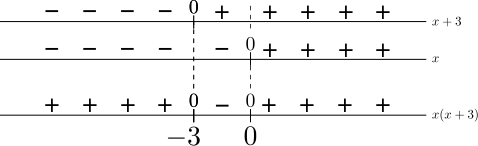
\includegraphics[width=0.7\textwidth]{19_c.png}
\end{figure}
	
Por lo tanto: $\text{Dom}\left(f(x)\right) = (-\infty,-3] \cup [0,+\infty)$.
	
\item Tenemos una función racional, y su dominio serán todos los números reales \textit{que no anulen el denominador} (\textit{¿por qué?}). Por lo tanto, debemos resolver: 
	
\[x^3 - x^2 \neq 0 \implies x^2(x - 1) \neq 0.\]
	
Esta última expresión excluye del dominio a los valores $x = 0$ y $x = 1$. Por lo tanto: $\text{Dom}\left(f(x)\right) = (-\infty,0) \cup (0,1) \cup (1,+\infty)$.
	
\item Este ejercicio es similar al anterior, pero además debemos exigir la condición $\frac{x - 2}{x^3 - x^2} \geq 0$ para poder calcular la raíz cuadrada. Procedemos como antes, factorizando primero el denominador:
	
\[\frac{x - 2}{x^3 - x^2} = \frac{x - 2}{x^2(x - 1)} \geq 0.\]
	
En este caso, como $x^2$ es siempre positivo, podemos excluirlo del análisis de signos\footnote{Estrictamente, cuando hacemos esto estamos asumiendo que $x \neq 0$, porque el resultado de la nueva desigualdad \textit{sí incluye al cero}, y en ese sentido es diferente al resultado de la desigualdad original. Como vamos a excluir al cero más adelante, acá no nos importa mucho, \textit{pero es importante siempre prestar mucha atención cuando se hace alguna simplificación de este tipo}, ya que de lo contrario se podrían obtener resultados absurdos.} (\textit{¿por qué?}), y la desigualdad a resolver será:
	
\[\frac{x - 2}{x - 1} \geq 0,\]
	
y su diagrama de signos:

\begin{figure}[H]
	\centering
	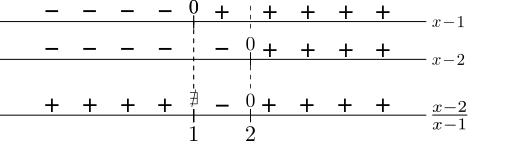
\includegraphics[width=0.8\textwidth]{19_e.png}
\end{figure}
	
Excluyendo los valores que anulan el denominador de la función original, es decir, $x = 0$ y $x = 1$ (calculados en el inciso anterior), resulta:
	
\[\text{Dom}\left(f(x)\right) = (-\infty,0) \cup (0,1) \cup [2,+\infty).\]
	
\begin{sloppypar}
\item La función $\log(x)$ tiene como dominio todos los reales positivos, y por lo tanto debemos exigir que su argumento sea estrictamente positivo, es decir, ${(2x + 3)(x - 1) > 0}$. El diagrama de signos es:
\end{sloppypar}

\begin{figure}[H]
	\centering
	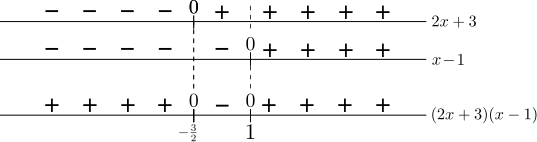
\includegraphics[width=0.8\textwidth]{19_f.png}
\end{figure}
	
Entonces:
	
\[\text{Dom}\left(f(x)\right) =\left(-\infty,-\frac{3}{2}\right) \cup (1,+\infty).\]

\end{enumerate}

%XXXXXXXXXXXXXXX  FABIAN

\section{Valor absoluto. El valor absoluto como distancia}


%19
\item \textbf{Ejercicio 20:}  Dar la interpretación geométrica del valor absoluto de un número real, interpretándolo en términos de distancia.\\
\textbf{R}: Esto está detallado en el  \href{https://youtu.be/IPX7iZAY6wk}{\textcolor{blue}{video 7}}, de la serie Conjuntos Numéricos, disponible en formato pdf también en \href{https://pedco.uncoma.edu.ar/}{\textcolor{blue}{ PEDCO}}.

%20
\item \textbf{Ejercicio 22:}  Interpretar las siguientes expresiones en términos de distancia, graficar y dar el conjunto solución (cuando corresponda) como intervalos o unión de  intervalos:

\begin{itemize}
\item Inciso \textit{(c)}  $|x-c| = 2$\\
\textbf{R}: La solución a esta ecuación es un conjunto formado por dos puntos:$\{c-2; c+2\}$, equidistantes dos unidades de $c$, uno a la izquierda y el otro a la derecha.  
\item  Inciso \textit{(g)}$|x-c| < 2$\\
\textbf{R}: La solución a esta inecuación es un conjunto formado por todos los puntos del intervalo $(c-2; c+2)$, centrado en $c$ y de radio 2.
\item  Inciso \textit{(h)} $|x-3| < d$\\
\textbf{R}: La solución a esta inecuación es un conjunto formado por todos los puntos del intervalo $(3-d; 3+d)$, centrado en $3$ y de radio d.
\item  Inciso \textit{(o)}  $|x| \geq 3$\\
\textbf{R}: La solución a esta inecuación es un conjunto formado por todos los puntos pertenecientes a la unión de intervalos $(-\infty;-3)\cup (3, +\infty)$.
\end{itemize}

\begin{figure}[H]
\centering
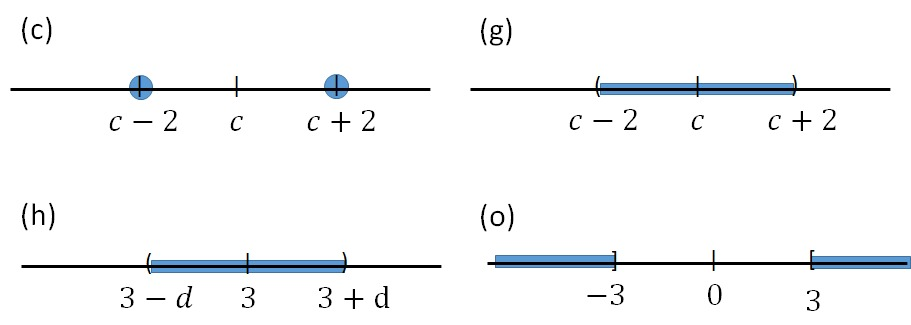
\includegraphics[width=0.9\textwidth]{20.png}
\end{figure}

%\begin{multicols}{4}
%\end{multicols}


%18
\item \textbf{Ejercicio 23:} Considerar los siguientes conjuntos. Primero graficar y pensarlos en términos de distancia. Luego escribir simbólicamente esa distancia usando el módulo.\\
\textbf{R}: Gráficos:\\

\begin{figure}[H]
\centering
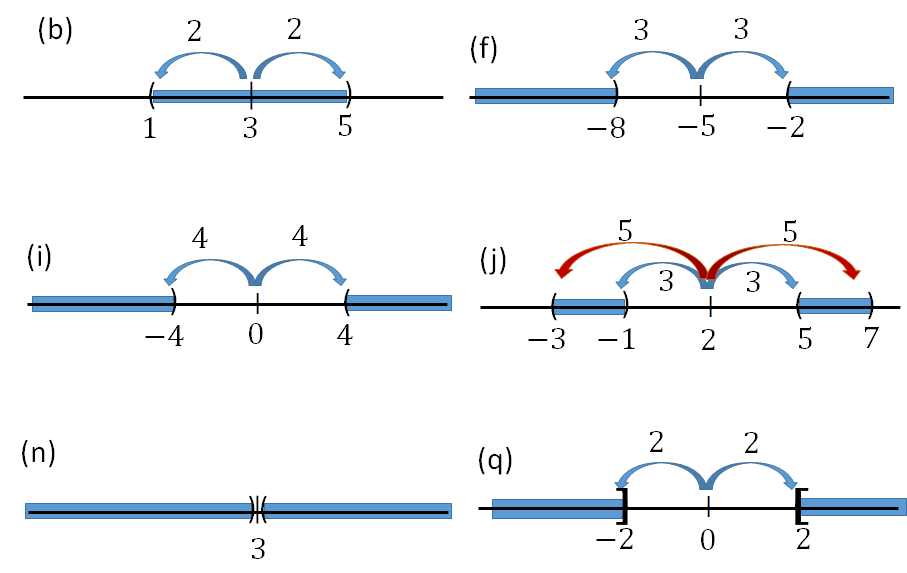
\includegraphics[width=0.9\textwidth]{23.png}
\end{figure}
\begin{itemize}
\setlength\itemsep{0em}
\item Inciso \textit{(b)}Puntos de la recta que distan de $3$ en menos de $2$ unidades.\\
\textbf{R}: $|x-3| < 2$
\item Inciso \textit{(f)}Puntos de la recta que distan de $-5$ en más de $3$ unidades.\\
\textbf{R}:  $|x-(-5)| =  |x+5|>3 $
\item Inciso \textit{(i)}Puntos de la recta que distan de $0$ en más de $4$ unidades.\\
\textbf{R}:  $|x| >4$
\item Inciso \textit{(j)}Puntos de la recta que distan de $2$ en  menos de  $5$ y más de $3$ unidades.\\
\textbf{R}:  $3< |x-2| < 5$. Esto puede escribirse también como  $|x-2| >3$ y  $|x-2| < 5$, entendiéndose que el conectivo es un conectivo lógico.
\item Inciso \textit{(n)}$\{ x \in \mathbb{R}$ tales  que $x \neq 3\}$\\
\textbf{R}:  $|x-3| >0$
\item Inciso \textit{(q)}$\{ x \in \mathbb{R}$ tales  que $x \in (- \infty, -2] \cup [2, +\infty)\}$\\
\textbf{R}:  $|x| \geq 2$
\end{itemize}

%%%%%%%%%%


\section{Función valor absoluto}

%26
\item \textbf{Ejercicio 26:} 
Vamos a resolver en este ejercicio los incisos (e), (k) y (l). Haremos en cada uno lo pedido.
\begin{itemize}
\item Inciso \textit{(b)} $f(x) = \sin x$ si $x \in [0, 2\pi]$

\begin{enumerate}
\begin{multicols}{2}
\item Graficar $f(x)$ 
\begin{figure}[H]
\centering
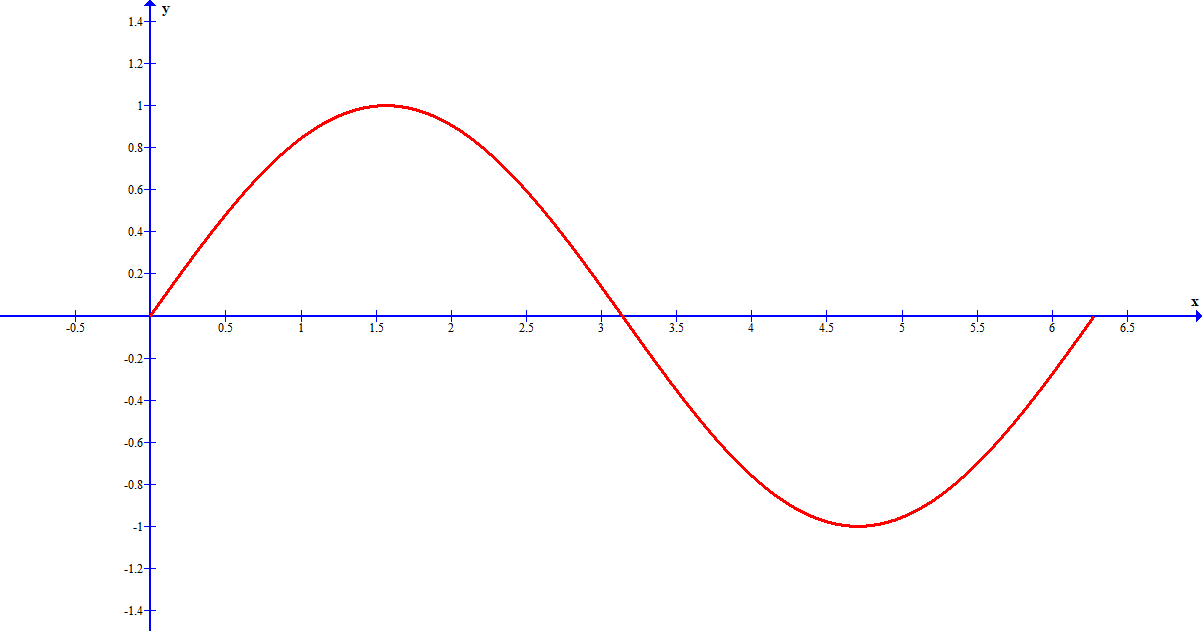
\includegraphics[width=0.45\textwidth]{26-1.png}
\end{figure}
\item Graficar $|f(x)|$ y llamarla $g(x)$ 
\begin{figure}[H]
\centering
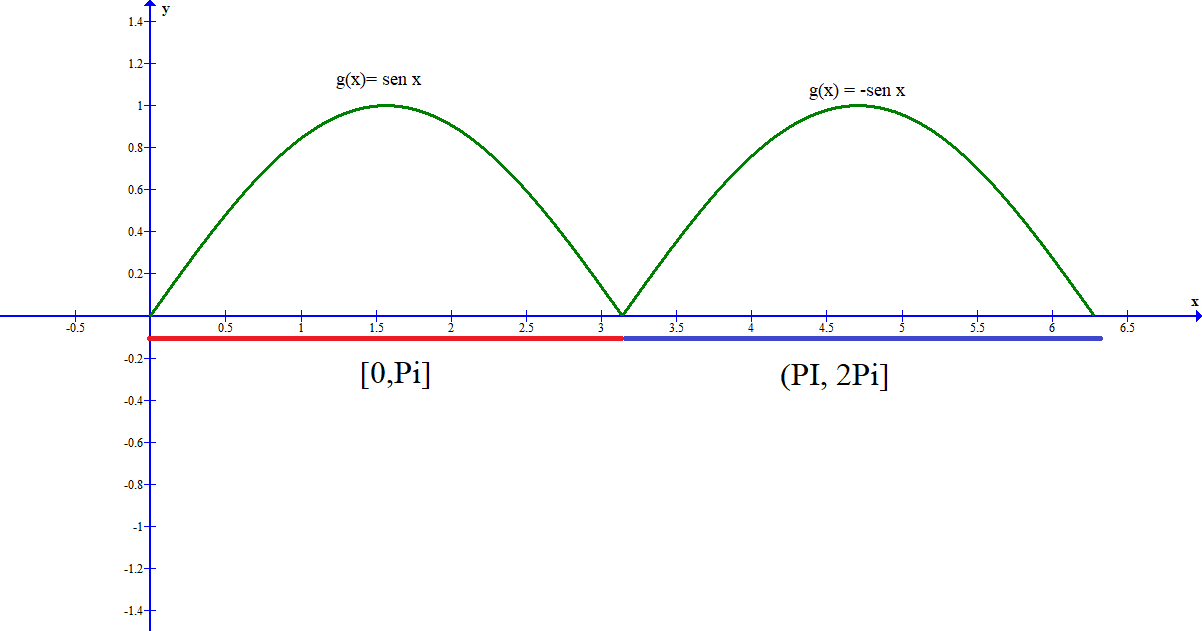
\includegraphics[width=0.45\textwidth]{26-2.png}
\end{figure}
\end{multicols}

\item En la función módulo, indicar sobre el gráfico, cuál es el valor de la función en cada intervalo del dominio definido por el módulo. Nombrar esos intervalos.\\
\textbf{R}: Como está indicado en el gráfico de la derecha, en el intervalo $[0, \pi]$ la función $g(x) = f(x) = sen(x)$ y en $(\pi, 2\pi]$ la función
$g(x) = -f(x) = -sen(x)$  
\item Desdoblar el módulo de acuerdo a la definición y comparar con lo analizado en el inciso anterior\\
\textbf{R}: 
\begin{equation*}
         g(x) = | f(x) | = \left \{
	\begin{aligned}
	sen(x)  \text{   si }  x \in  [0, \pi]\\
	-sen(x) \text{ si } x \in  (\pi, 2\pi]
	\end{aligned}
	\right.
\end{equation*}
\end{enumerate}
%}
\item Inciso \textit{(b)}: $f(x) = x.(x-1).(x+1)$
\begin{enumerate}
\begin{multicols}{2}
\item Graficar $f(x)$ 
\begin{figure}[H]
\centering
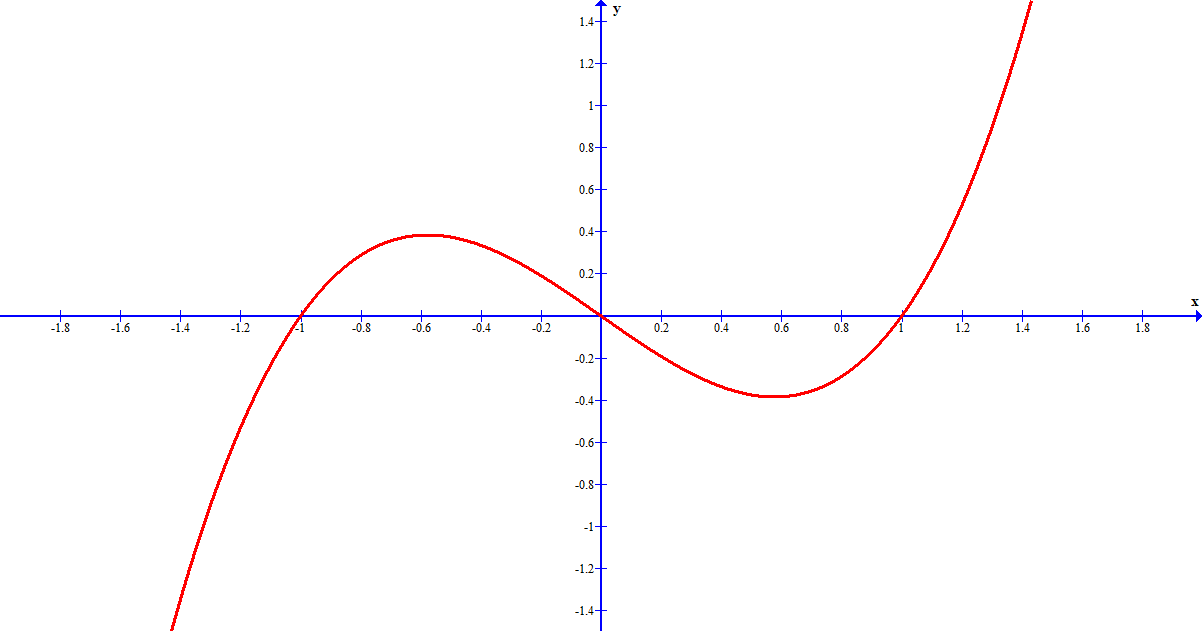
\includegraphics[width=0.45\textwidth]{26-3.png}
\end{figure}

\item Graficar $|f(x)|$ y llamarla $g(x)$ 
\begin{figure}[H]
\centering
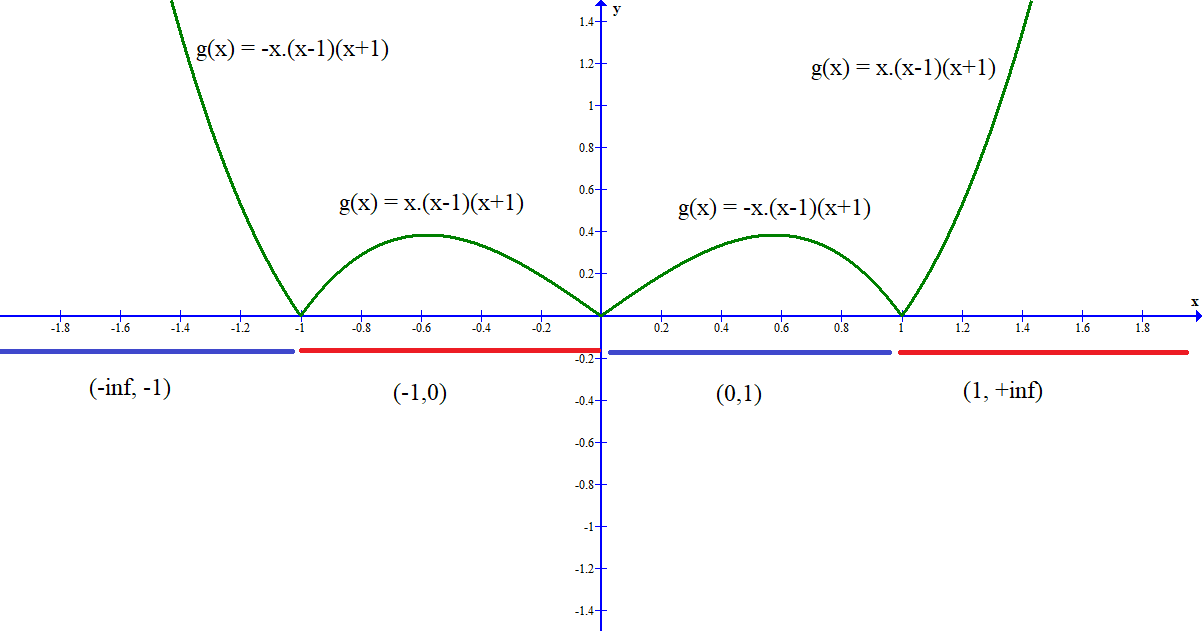
\includegraphics[width=0.45\textwidth]{26-4.png}
\end{figure}
\end{multicols}

\item En la función módulo, indicar sobre el gráfico, cuál es el valor de la función en cada intervalo del dominio definido por el módulo. Nombrar esos intervalos.\\
\textbf{R}: Como está indicado en el gráfico de la derecha, en $(-\infty,-1) \cup (0,1) $ la función $g(x) = -f(x) = -x(x-1)(x+1)$ y en $[-1,0] \cup [1, +\infty)$ la función $g(x) = f(x) = x.(x-1)(x+1)$  
\item Desdoblar el módulo de acuerdo a la definición y comparar con lo analizado en el inciso anterior\\
\textbf{R}: 
\begin{equation*}
         g(x) = | f(x) | = \left \{
	\begin{aligned}
	x(x-1)(x+1)  \text{   si }  x \in  [-1,0] \cup [1, +\infty)\\
	-x(x-1)(x+1) \text{ si } x \in  (-\infty,-1) \cup (0, 1)
	\end{aligned}
	\right.
\end{equation*}
\end{enumerate}

\item Inciso \textit{(b)}: $f(x) =  \ln(x)$  
\begin{enumerate}
\begin{multicols}{2}
\item Graficar $f(x)$ 
\begin{figure}[H]
\centering
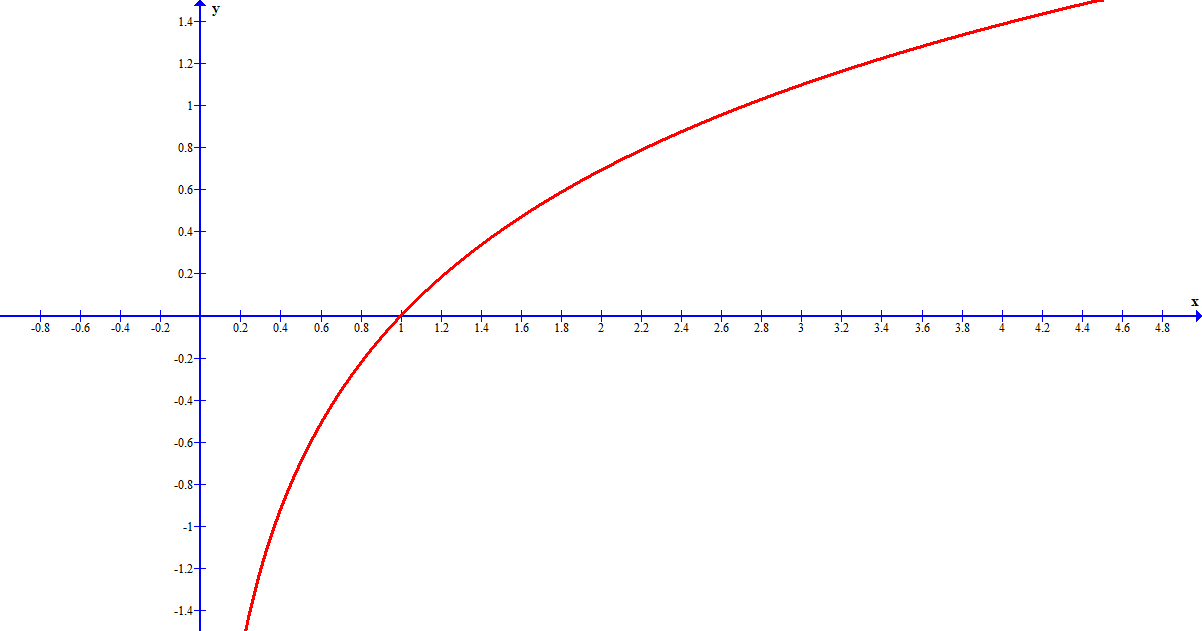
\includegraphics[width=0.45\textwidth]{26-5.png}
\end{figure}
\item Graficar $|f(x)|$ y llamarla $g(x)$ 
\begin{figure}[H]
\centering
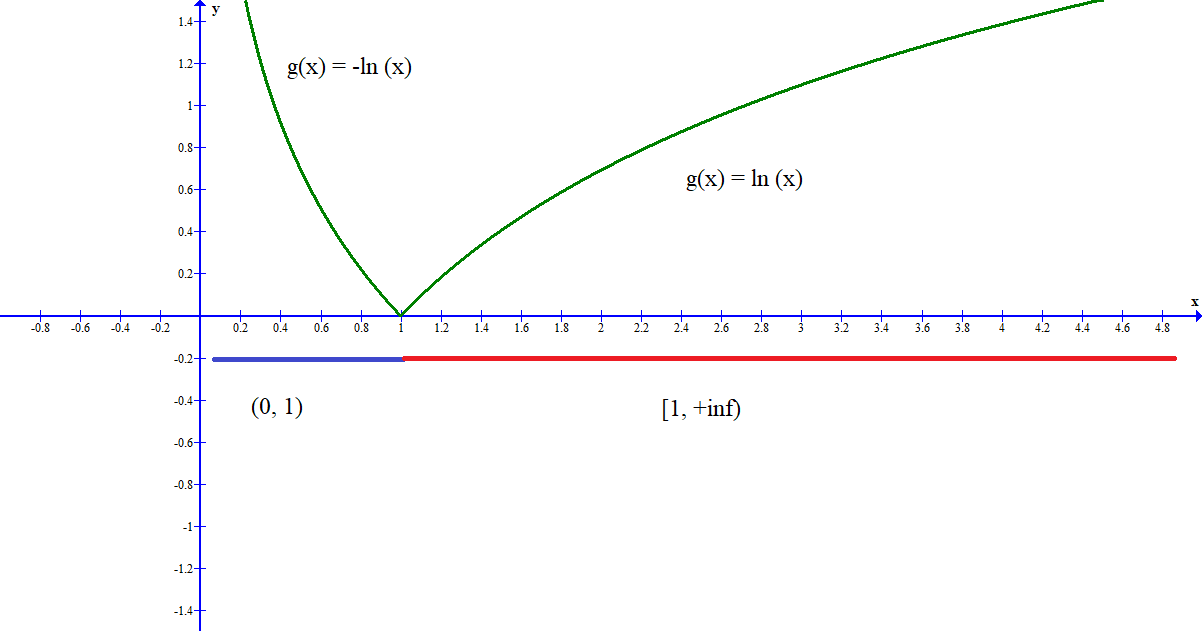
\includegraphics[width=0.45\textwidth]{26-6.png}
\end{figure}
\end{multicols}

\item En la función módulo, indicar sobre el gráfico, cuál es el valor de la función en cada intervalo del dominio definido por el módulo. Nombrar esos intervalos.\\
\textbf{R}:  Como está indicado en el gráfico.
\item Desdoblar el módulo de acuerdo a la definición y comparar con lo analizado en el inciso anterior\\
\textbf{R}: 
\begin{equation*}
         g(x) = | f(x) | = \left \{
	\begin{aligned}
	ln (x)  \text{   si }  x \in  [1,+ \infty)\\
	-ln (x) \text{ si } x \in  (0,1)
	\end{aligned}
	\right.
\end{equation*}
\end{enumerate}
\end{itemize}

\item  \textbf{Ejercicio 27:}  Hallar los valores de $x$ que satisfacen las siguientes expresiones, interpretándolas gráficamente como comparación de funciones:\\
Resolveremos el inciso \textit{(c)}: $|2x-4| \geq 3$ 
\begin{figure}[H]
\centering
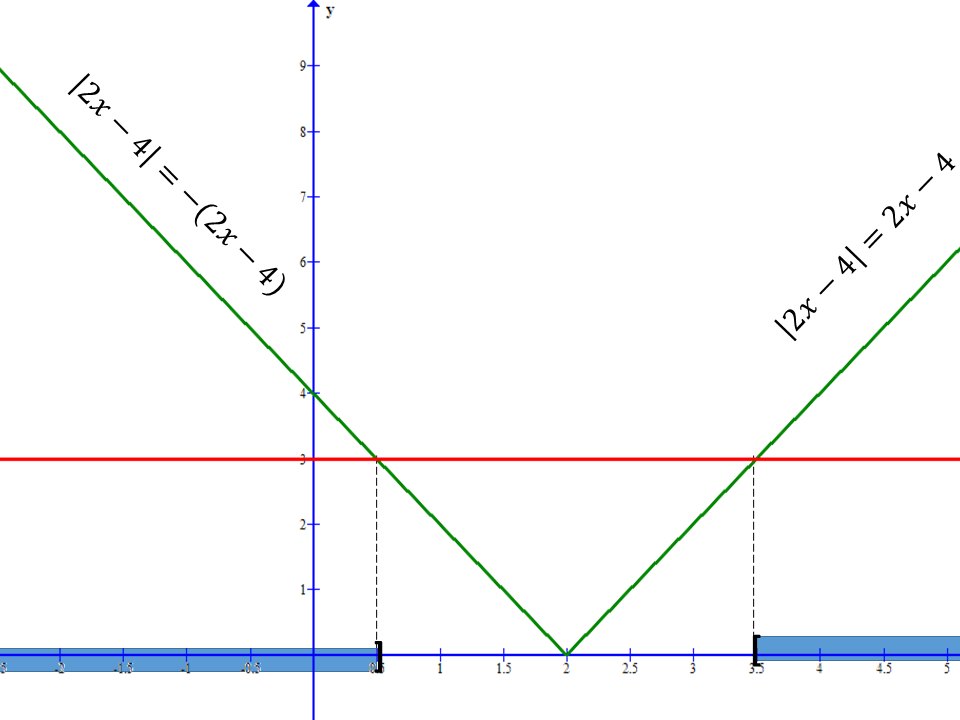
\includegraphics[width=0.8\textwidth]{27.png}
\end{figure}
Llamemos $|f(x)|$ a la función de la izquierda y $g(x)$ a la de la derecha. La primera función será entonces:
\begin{equation*}
         | fx | = \left \{
	\begin{aligned}
	2x-4  \text{   si }  x \in  [2,+ \infty)\\
	-(2x-4) \text{ si } x \in  (-\infty, 2)
	\end{aligned}
	\right.
\end{equation*}

La solución de esta desigualdad es una unión de intervalos $(-\infty, x_0] \cup [x_1, + \infty)$. Debemos encontrar analíticamente los valores $x_0$ y $x_1$. El primero es el resultado de la intersección de $|f(x)| = -(2x-4)$ con g(x) y el segundo, de  $|f(x)| = (2x-4)$ con g(x).\\
Tenemos entonces:\\
$-(2x-4)= 3$ entonces $-2x = 3-4$, por lo que $x = 0,5$\\
Análogamente:\\
$2x-4= 3$ entonces $2x = 3+4$, por lo que $x =3,5$\\
La solución de la desigualdad es entonces s $(-\infty; 0,5] \cup [3,5 ; + \infty)$


\item   \textbf{Ejercicio 30:} Considerar las funciones  $|f(x)| = |x^{2}-4|$ y $g(x) = 2x-1$
\begin{enumerate}
\item realizar un gráfico de ambas funciones (mejor en un mismo gráfico)
\item Para $|f(x)|$ definir la función en cada tramo del gráfico (es decir, a qué es igual $|f(x)|$ según si las imágenes de $f(x)$ son positivas o negativas)
\item Encontrar los puntos de intersección entre $|f(x)|$ y $g(x)$ (analíticamente)
\item Señalar en el eje $x$ de este gráfico, el conjunto de puntos para los cuales es $|f(x)| \geq g(x)$.
\item Escribir lo anterior usando intervalos (o unión de ellos)
\end{enumerate}
\textbf{R}: Este ejercicio está resuelto en detalle el video del \href{https://youtu.be/myuKj55l_jg }{\textcolor{blue}{Octavo encuentro virtual}} disponible en formato pdf también en \href{https://pedco.uncoma.edu.ar/}{\textcolor{blue}{ PEDCO}}.


\item  \textbf{Ejercicio 31:} Analizaremos tres de las desigualdades propuestas
\begin{itemize}
%primera
\item  Inciso \textit{(c)} $3x-4 <|5x-1| $\\
Llamemos $f(x) = 3x-4 $ y $|g(x)| = |5x-1| $
	\begin{enumerate}
	\item Graficar las funciones que representan cada lado de la desigualdad
	\begin{figure}[H]
	\centering
	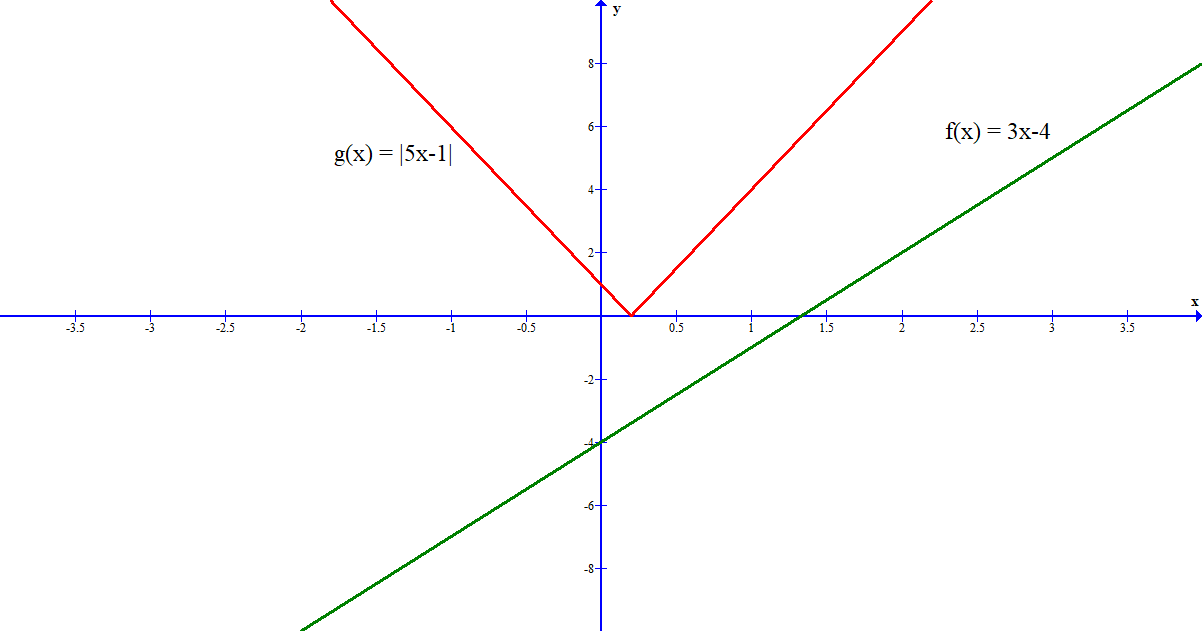
\includegraphics[width=0.7\textwidth]{31-1.png}
	\end{figure}
	\item Proceder como en el ejercicio anterior para determinar el conjunto solución\\
	\textbf{R}: En este caso en particular, la función $f(x) =3x-4$ está siempre por debajo de la función$ |g(x)| =|5x-1| $, por lo tanto el conjunto solución es todo $\mathbb{R}$.
	\end{enumerate}
%segunda
\item Inciso \textit{(e)}: $ |2x-1|\geq x^{2}+2 $
	Llamemos $|f(x)| =  |2x-1| $ y $g(x) = x^{2}+2 $
	\begin{enumerate}
	\item Graficar las funciones que representan cada lado de la desigualdad
	\begin{figure}[H]
	\centering
	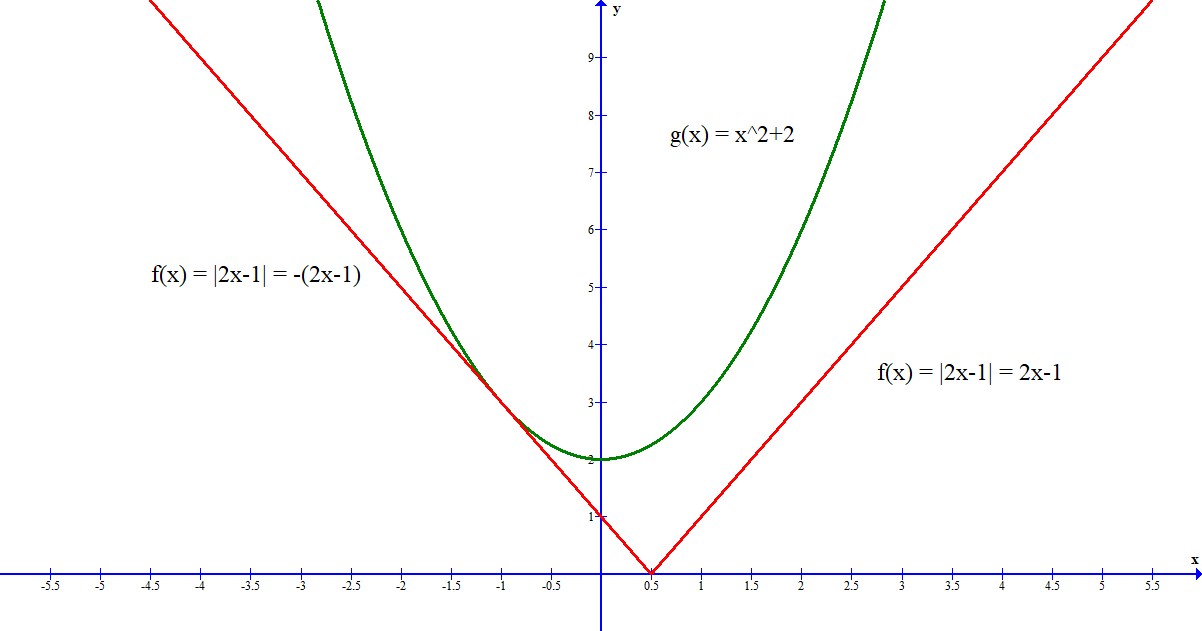
\includegraphics[width=0.7\textwidth]{31-2.png}
	\end{figure}
	\item Proceder como en el ejercicio anterior para determinar el conjunto solución\\
	\textbf{R}: En este caso en particular, la función $|f(x)| =|2x-1|$ está siempre por debajo de la función$ g(x) =x^{2}+2 $, excepto en el punto de intersección, donde son iguales. La consigna requiere encontrar el conjunto de números reales para los 	cuales $|f(x)|$ es mayor o igual que $g(x)$. El caso \textit{mayor} no ocurre nunca. Solo ocurre el caso \textit{igual}, por lo tanto el conjunto solución se reduce al único punto de intersección, que se encuentra analíticamente:\\
	El punto de contacto de las funciones ocurre donde las imágenes de $f(x) = 2x-1$ son negativas, por lo que $|f(x)| =|2x-1|= 			-(2x-1)$. Debemos resolver entonces la igualdad:\\
	$ x^{2}+2 = -(2x-1)$ \\
	$ x^{2}+2  +2x-1 = 0$\\
	$ x^{2}+2x+1 = 0$ \\
	La única solución de esta ecuación es $x=-1$, por lo que el conjunto solución de la desigualdad es $S = {-1}$.
	\end{enumerate}
%tercera
	\item Inciso \textit{(g)}: $ |x^{2}-4 |\leq -2x + 4$
	\begin{enumerate}
	\item Graficar las funciones que representan cada lado de la desigualdad
	\begin{figure}[H]
	\centering
	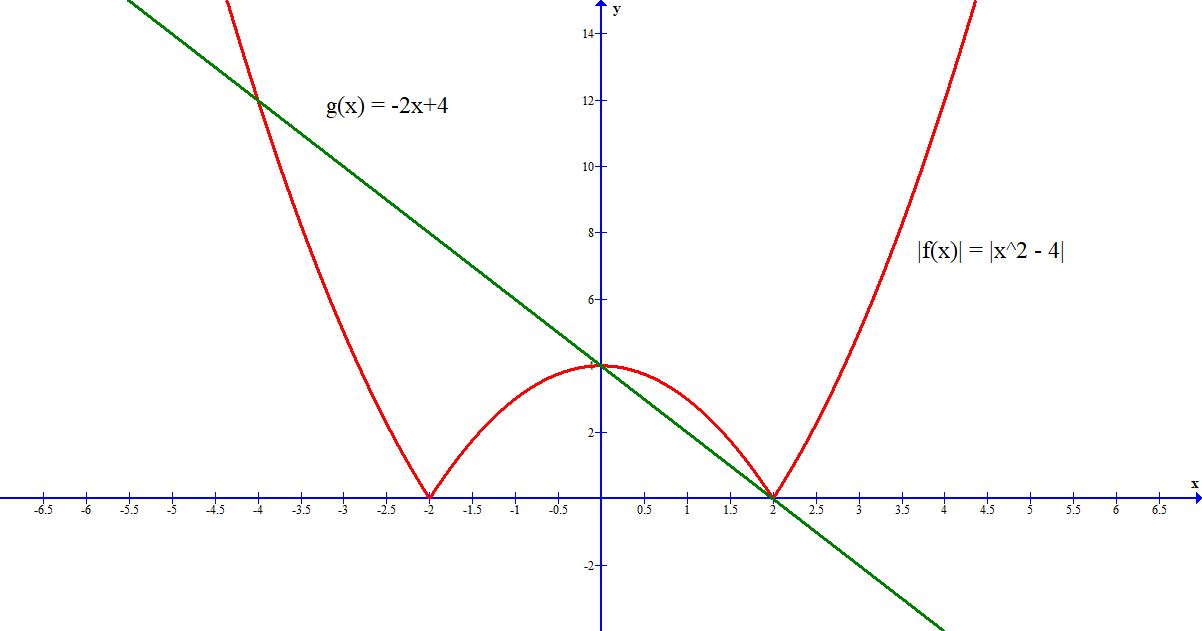
\includegraphics[width=0.7\textwidth]{31-3.png}
	\end{figure}
	\item Proceder como en el ejercicio anterior para determinar el conjunto solución\\
	\textbf{R}: En el gráfico se ve que  $ |x^{2}-4 |\leq -2x+4 $ en un intervalo $[x_0,x_1]$, incluyendo los bordes porque se 			trata de una desigualdad amplia, y además, las dos curvas se vuelven a cortar en un punto a la derecha de cero.
	El límite inferior del intervalo es el punto de intersección de $f(x) =|x^{2}-4| =  x^{2}-4$ con la recta $g(x) = -2x+4 $. Para 			buscar este punto debemos resolver la ecuación: \\
	$x^{2}-4= -2x+4 $\\
	$ x^{2}-4 +2x-4=0 $\\
	$x^{2}+2x-8=0$\\
	$(x+4)(x-2)=0$\\
	De las dos raíces de esta ecuación nos sirve $x=-4$ que delimita por la izquierda el conjunto solución.\\
	Para el límite superior del intervalo, debemos resolver la  la ecuación: \\
	$-(x^{2}-4)= -2x+4 $\\
	$ -x^{2}+4 +2x-4=0 $\\
	$-x^{2}+2x=0$\\
	$-x(x-2)=0$\\
	\end{enumerate}
	El extremo superior del intervalo es $x=0$.
	Ambas ecuaciones también dan como resultado el punto $x=2$, que es también parte de la solución porque en ese punto se 			cumple la condición de igualdad. Por lo que el conjunto solución de la desigualdad es $S = [-4,0] \cup \{2\}$.

\item Inciso \textit{(h)}$ 2x-1 \geq |(2-x).x|$
           Llamemos $f(x) =  2x-1$ y $|g(x)| = |(2-x).x| $
	\begin{enumerate}
	\item Graficar las funciones que representan cada lado de la desigualdad
	\begin{figure}[H]
	\centering
	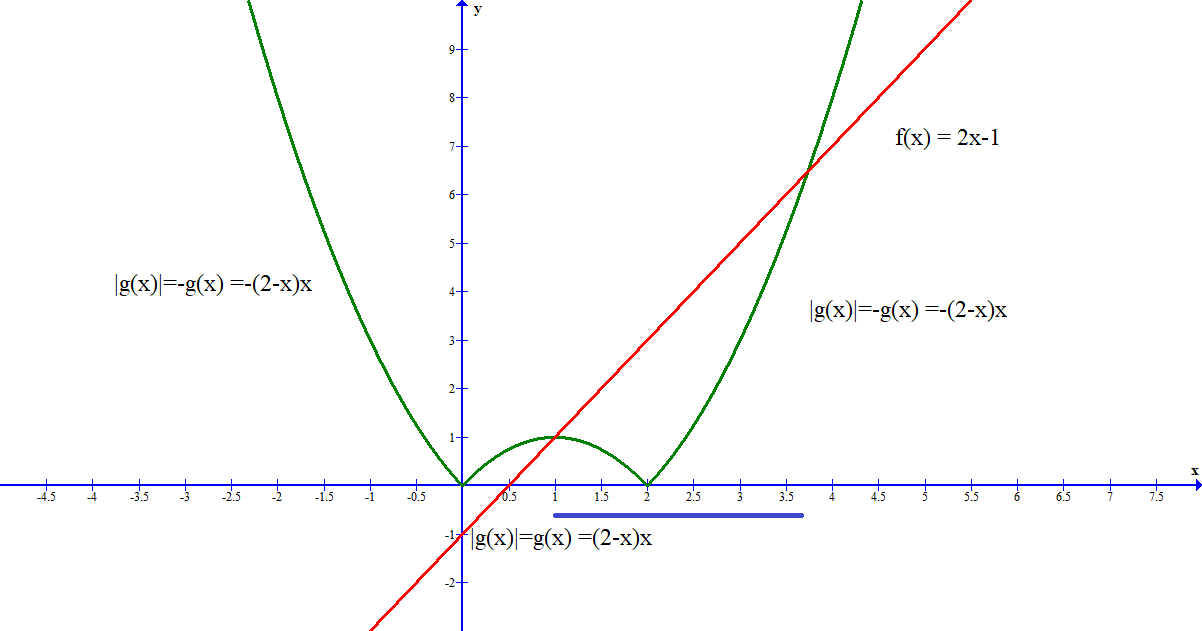
\includegraphics[width=0.7\textwidth]{31-4.png}
	\end{figure}
	\item Proceder como en el ejercicio anterior para determinar el conjunto solución\\
	\textbf{R}: En el gráfico se ve que $ 2x-1 \geq |(2-x).x|$en un intervalo $[x_0,x_1]$, incluyendo los bordes porque se 			trata de una desigualdad amplia. 
	El límite inferior del intervalo es el punto de intersección de la recta $f(x) =2x-1$ con  $|g(x)| = |(2-x).x| = (2-x).x$. Para hallar este punto debemos resolver la ecuación: \\
	$2x-1= (2-x).x $\\
	$2x-1-2x+x^{2}=0 $\\
	$x^{2}-1=0$\\
	$(x-1)(x+1)=0$\\
	De las dos raíces de esta ecuación nos sirve $x=1$ que delimita por la izquierda el conjunto solución.\\
	Para el límite superior del intervalo, debemos resolver la  la ecuación: \\
	$2x-1= -(2-x).x $\\
	$2x-1+2x-x^{2}=0 $\\
	$-x^{2}+4x-1=0$\\
	\end{enumerate}
	Esta ecuación cuadrática tiene dos raíces: $x \thicksim 3.732$ y  $x \thicksim 0.2679$. De estas dos raíces, la que está en el dominio de validez de nuestra ecuación, es la primera.\\
 Por lo tanto, el conjunto solución de la desigualdad es $S = [-1;3,732]$.

\end{itemize}

\end{enumerate}

\end{document}
